\documentclass{visionen-creative}
\usepackage{lipsum}
% Compile with LuaLaTeX. Keep visionen-creative.cls and the fonts/ directory
% next to this file. Replace the framed image placeholders with your images.
% A simple placeholder that keeps the example compilable without image files.
\newcommand{\ImagePlaceholder}[2]{%
  \fbox{%
    \parbox[c][#2][c]{\dimexpr\linewidth-2\fboxsep-2\fboxrule\relax}{%
      \centering\itshape #1
    }%
  }%
}
\ArticleStart{recto}
\begin{document}
% UNCOMMENT THIS LINE AS WELL AS THE NEXT LINE TO PUT YOUR ARTICLE'S START ON THE RIGHT SIDE OF THE SPREAD
%\newpage

\ArticleHeading
  {LaTeX Creative Article Template}
  {Hello Kitty - GET READY TO ROCK AND MRRREOWWWLLL!!!}
\OpeningParagraph{
You can format the opening paragraph like this, with a fancy three-line initial and first three words all-capped. However, make sure that the opening paragraph is sufficiently long to use this style, as the first letter \emph{has to} stretch over three lines of text. Of course, you're free to also not use this formatting and use the normal paragraph formatting for the opening instead.}
\vspace{8bp}
\hline
\vspace{6bp}
Paragraphs in this template are not indented, in contrast to the two-column template for text-heavy articles. The horizontal line is just for testing. If you want to have some space between paragraphs, use the \texttt{vspace} command with 8-12bp spacing.

\vspace{12bp}

% First composition: 6/10 text on the left, 4/10 image on the right.
\TextImageLayout{%
\vspace{12bp}
  \section*{A template for less text-heavy articles}
  This template is for articles that want to include images alongside text. Unlike the other template, this template only has left-justified text.

  The image in the image section is aligned to the top of the line of the text section, but you can use \texttt{vspace} to adjust the exact placement of either the text or the image, depending on the size of the text, size and shape of the image and on how big you want your caption to be.
}{%
  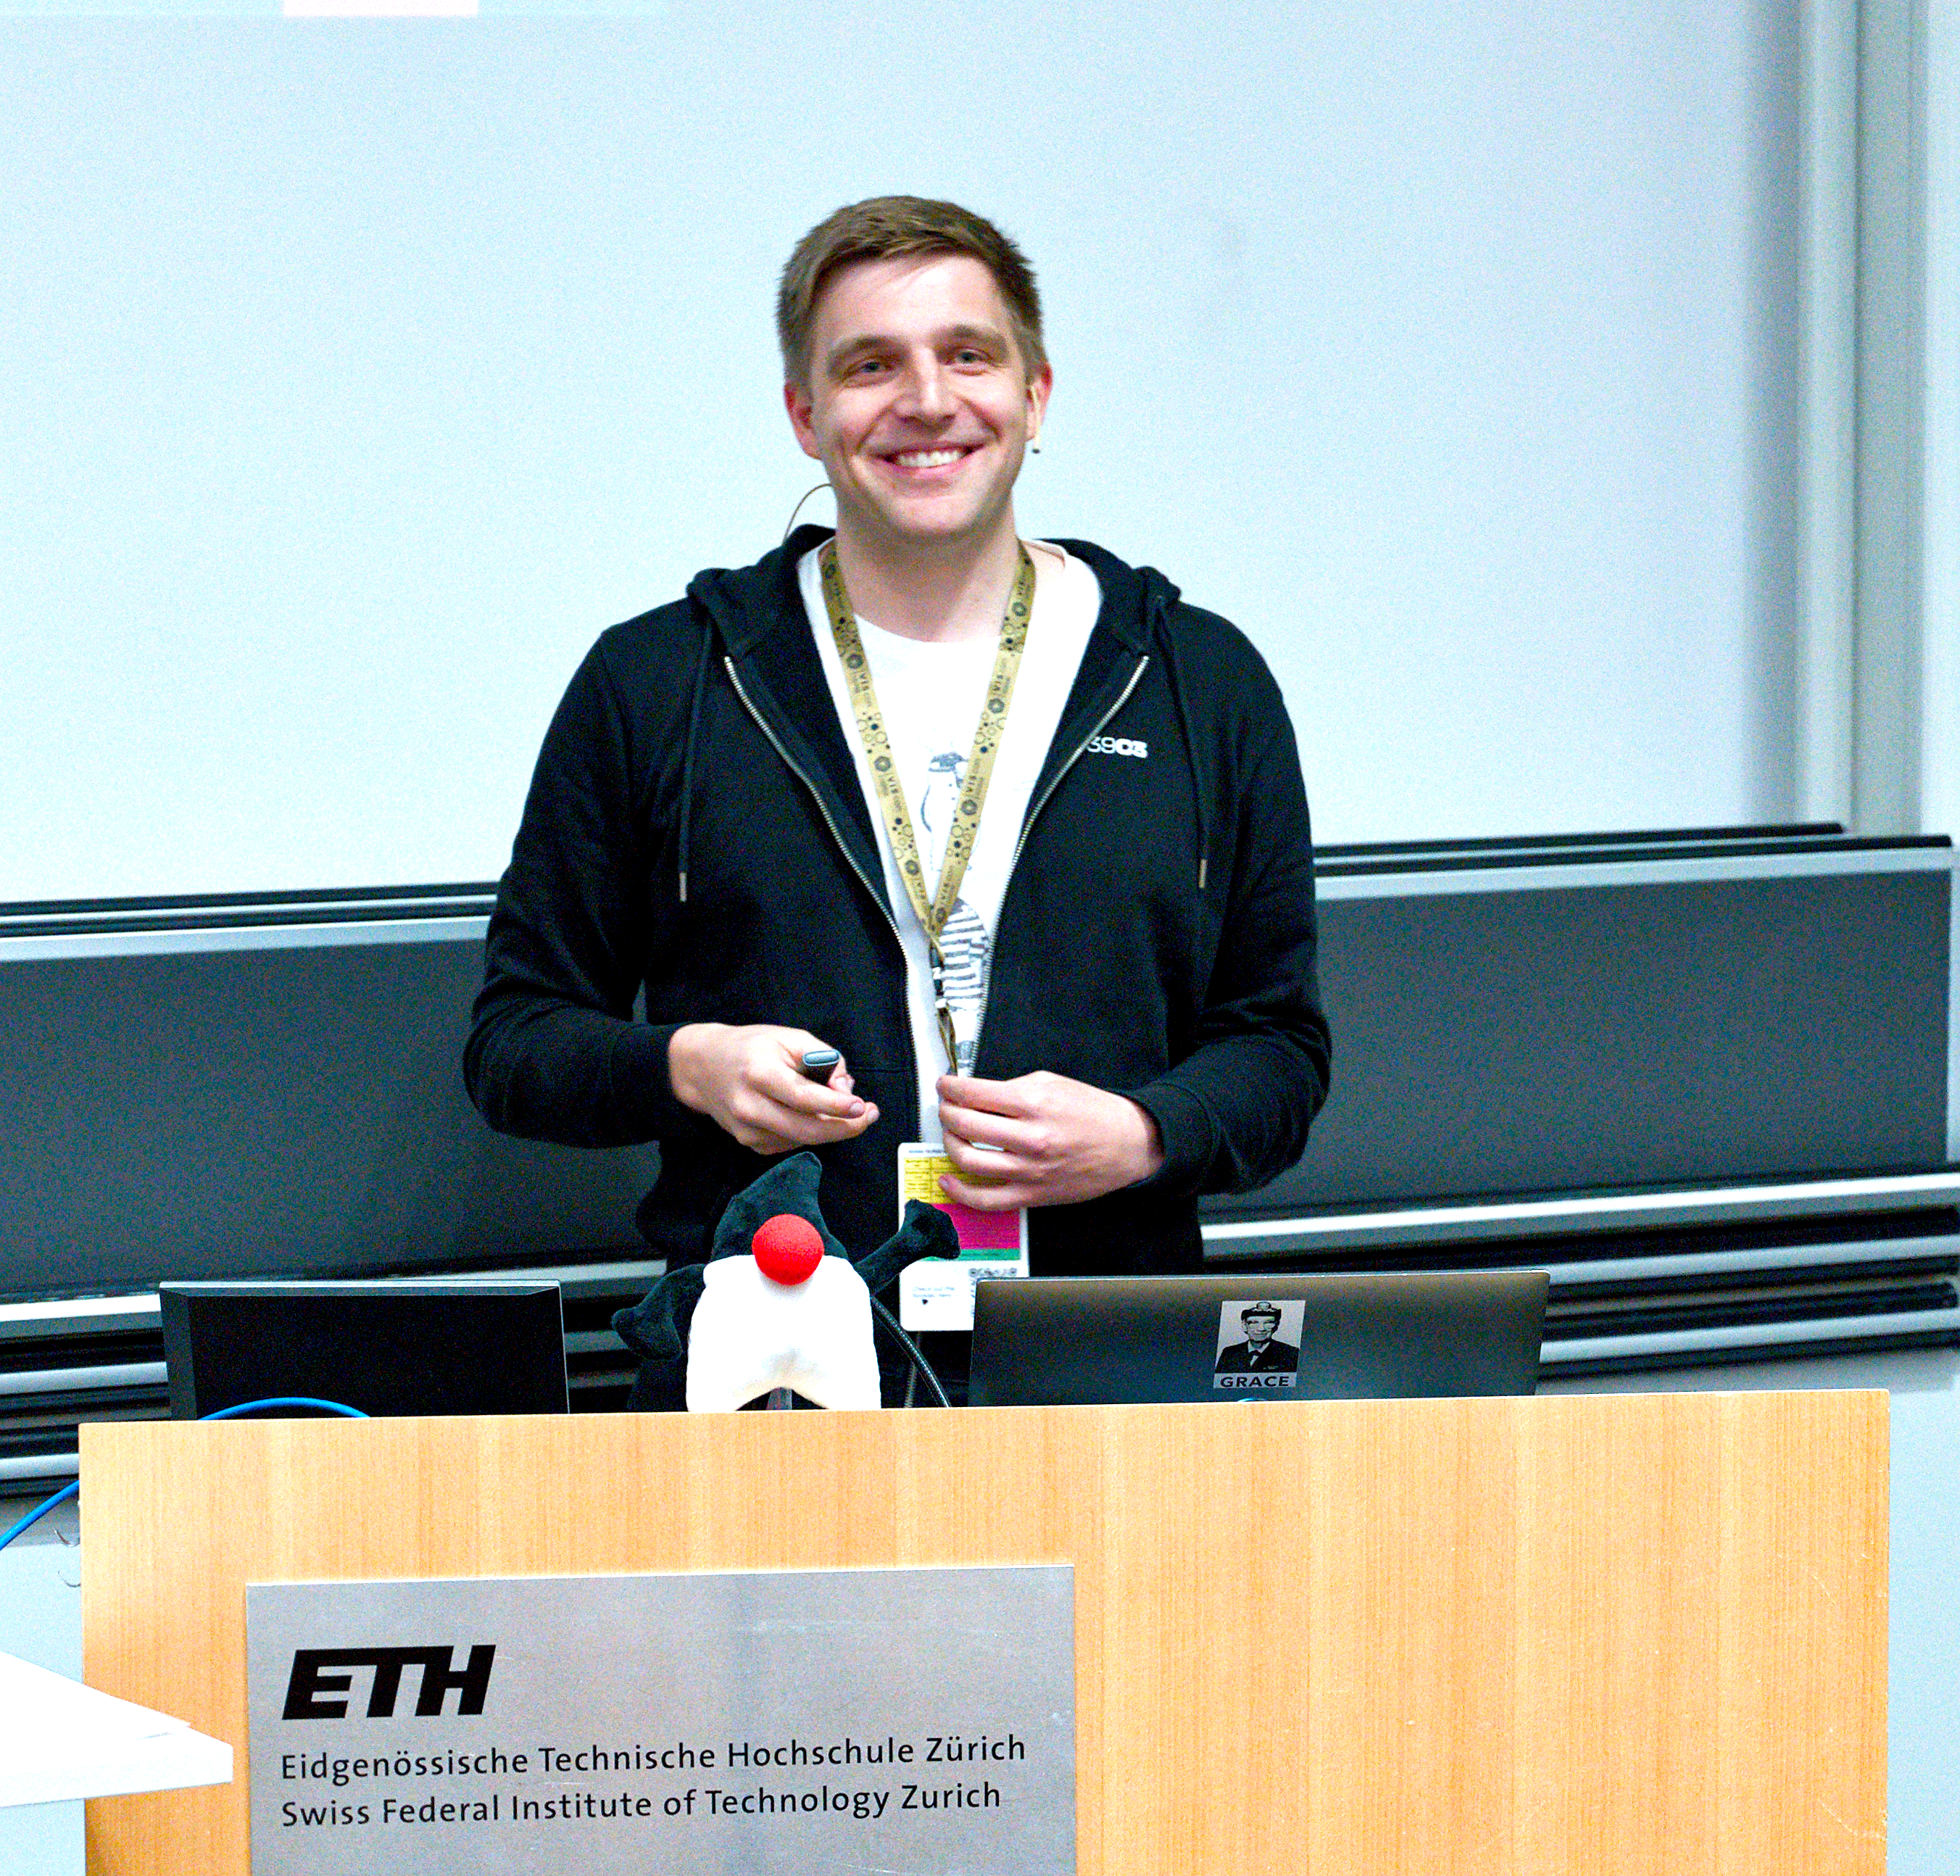
\includegraphics[width=\linewidth]{../images/VIScon_RaffaelStefanBischoff_21.jpg}
  %\ImagePlaceholder{Street photograph\\replace with image}{50mm} %edit the number here to adjust height
  \begin{Caption}{0bp}
    Make sure to crop your image beforehand and use \texttt{vspace} to get the image to fit the way you want it to.
  \end{Caption}
}

\vspace{12bp}

% Second composition: image on the left, 6/10 text on the right.
\ImageTextLayout{%
  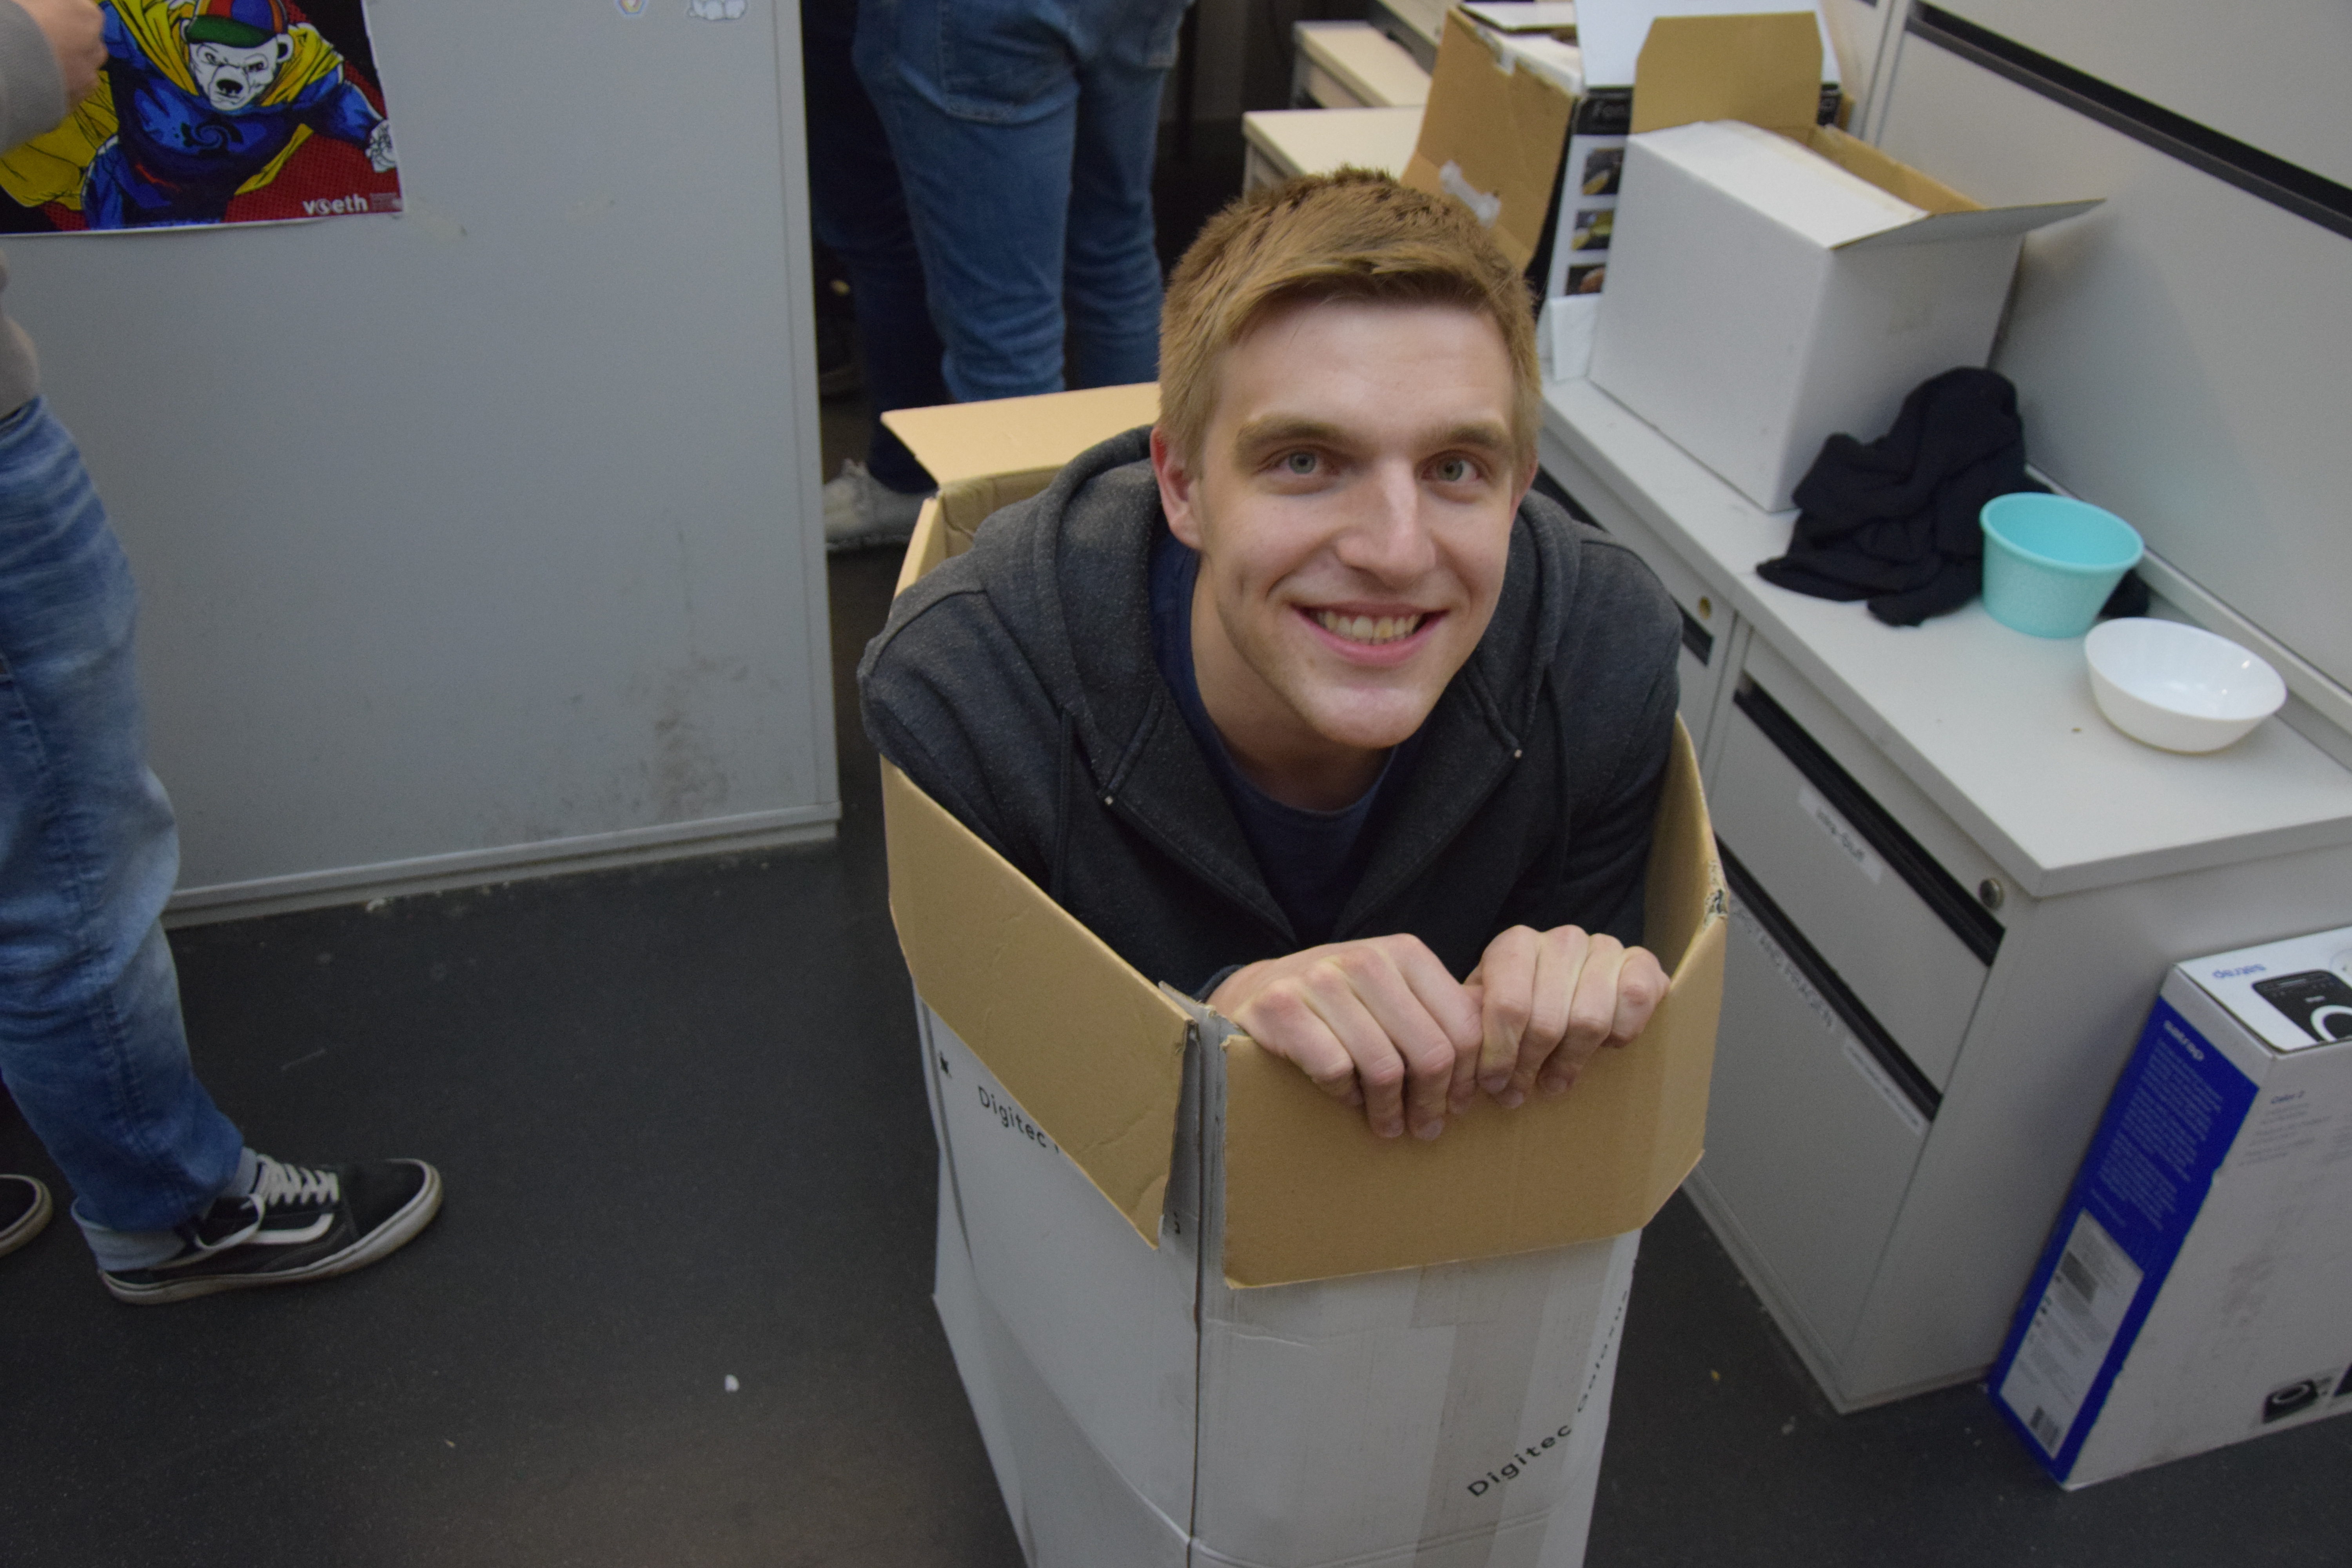
\includegraphics[width=\linewidth]{../images/DSC_0147.JPG}
  %\ImagePlaceholder{Public-space photograph\\replace with image}{50mm}
  \begin{Caption}{0bp}
    The cropping for this image is somewhat suboptimal. So I'm yapping to compensate.
  \end{Caption}
}{%
  \section*{Precautions}
  The proportions of text section to image section are 3:2 or 60-40. You are still able to include images in the center outside of 
  The \texttt{ImageTextLayout} element expects all elements to fit within the same page. Otherwise, all is put into the next page. 
  
Tip: Text that doesn't \emph{have} to be formatted in the text block can just be written as separate lines or paragraphs outside the element's curly brackets.
}

 A clear layout allows these activities to happen alongside one another. Blablabla inbetweener text for testing.

 
\ImageTextLayout{%
\vspace{24bp}\includegraphics[width=0]{}Testing text on the 40\% side... yep, you're able to reverse the pattern, using a funny quirk of putting images on both sections, but setting the 40\% side's image width to zero.
}
  {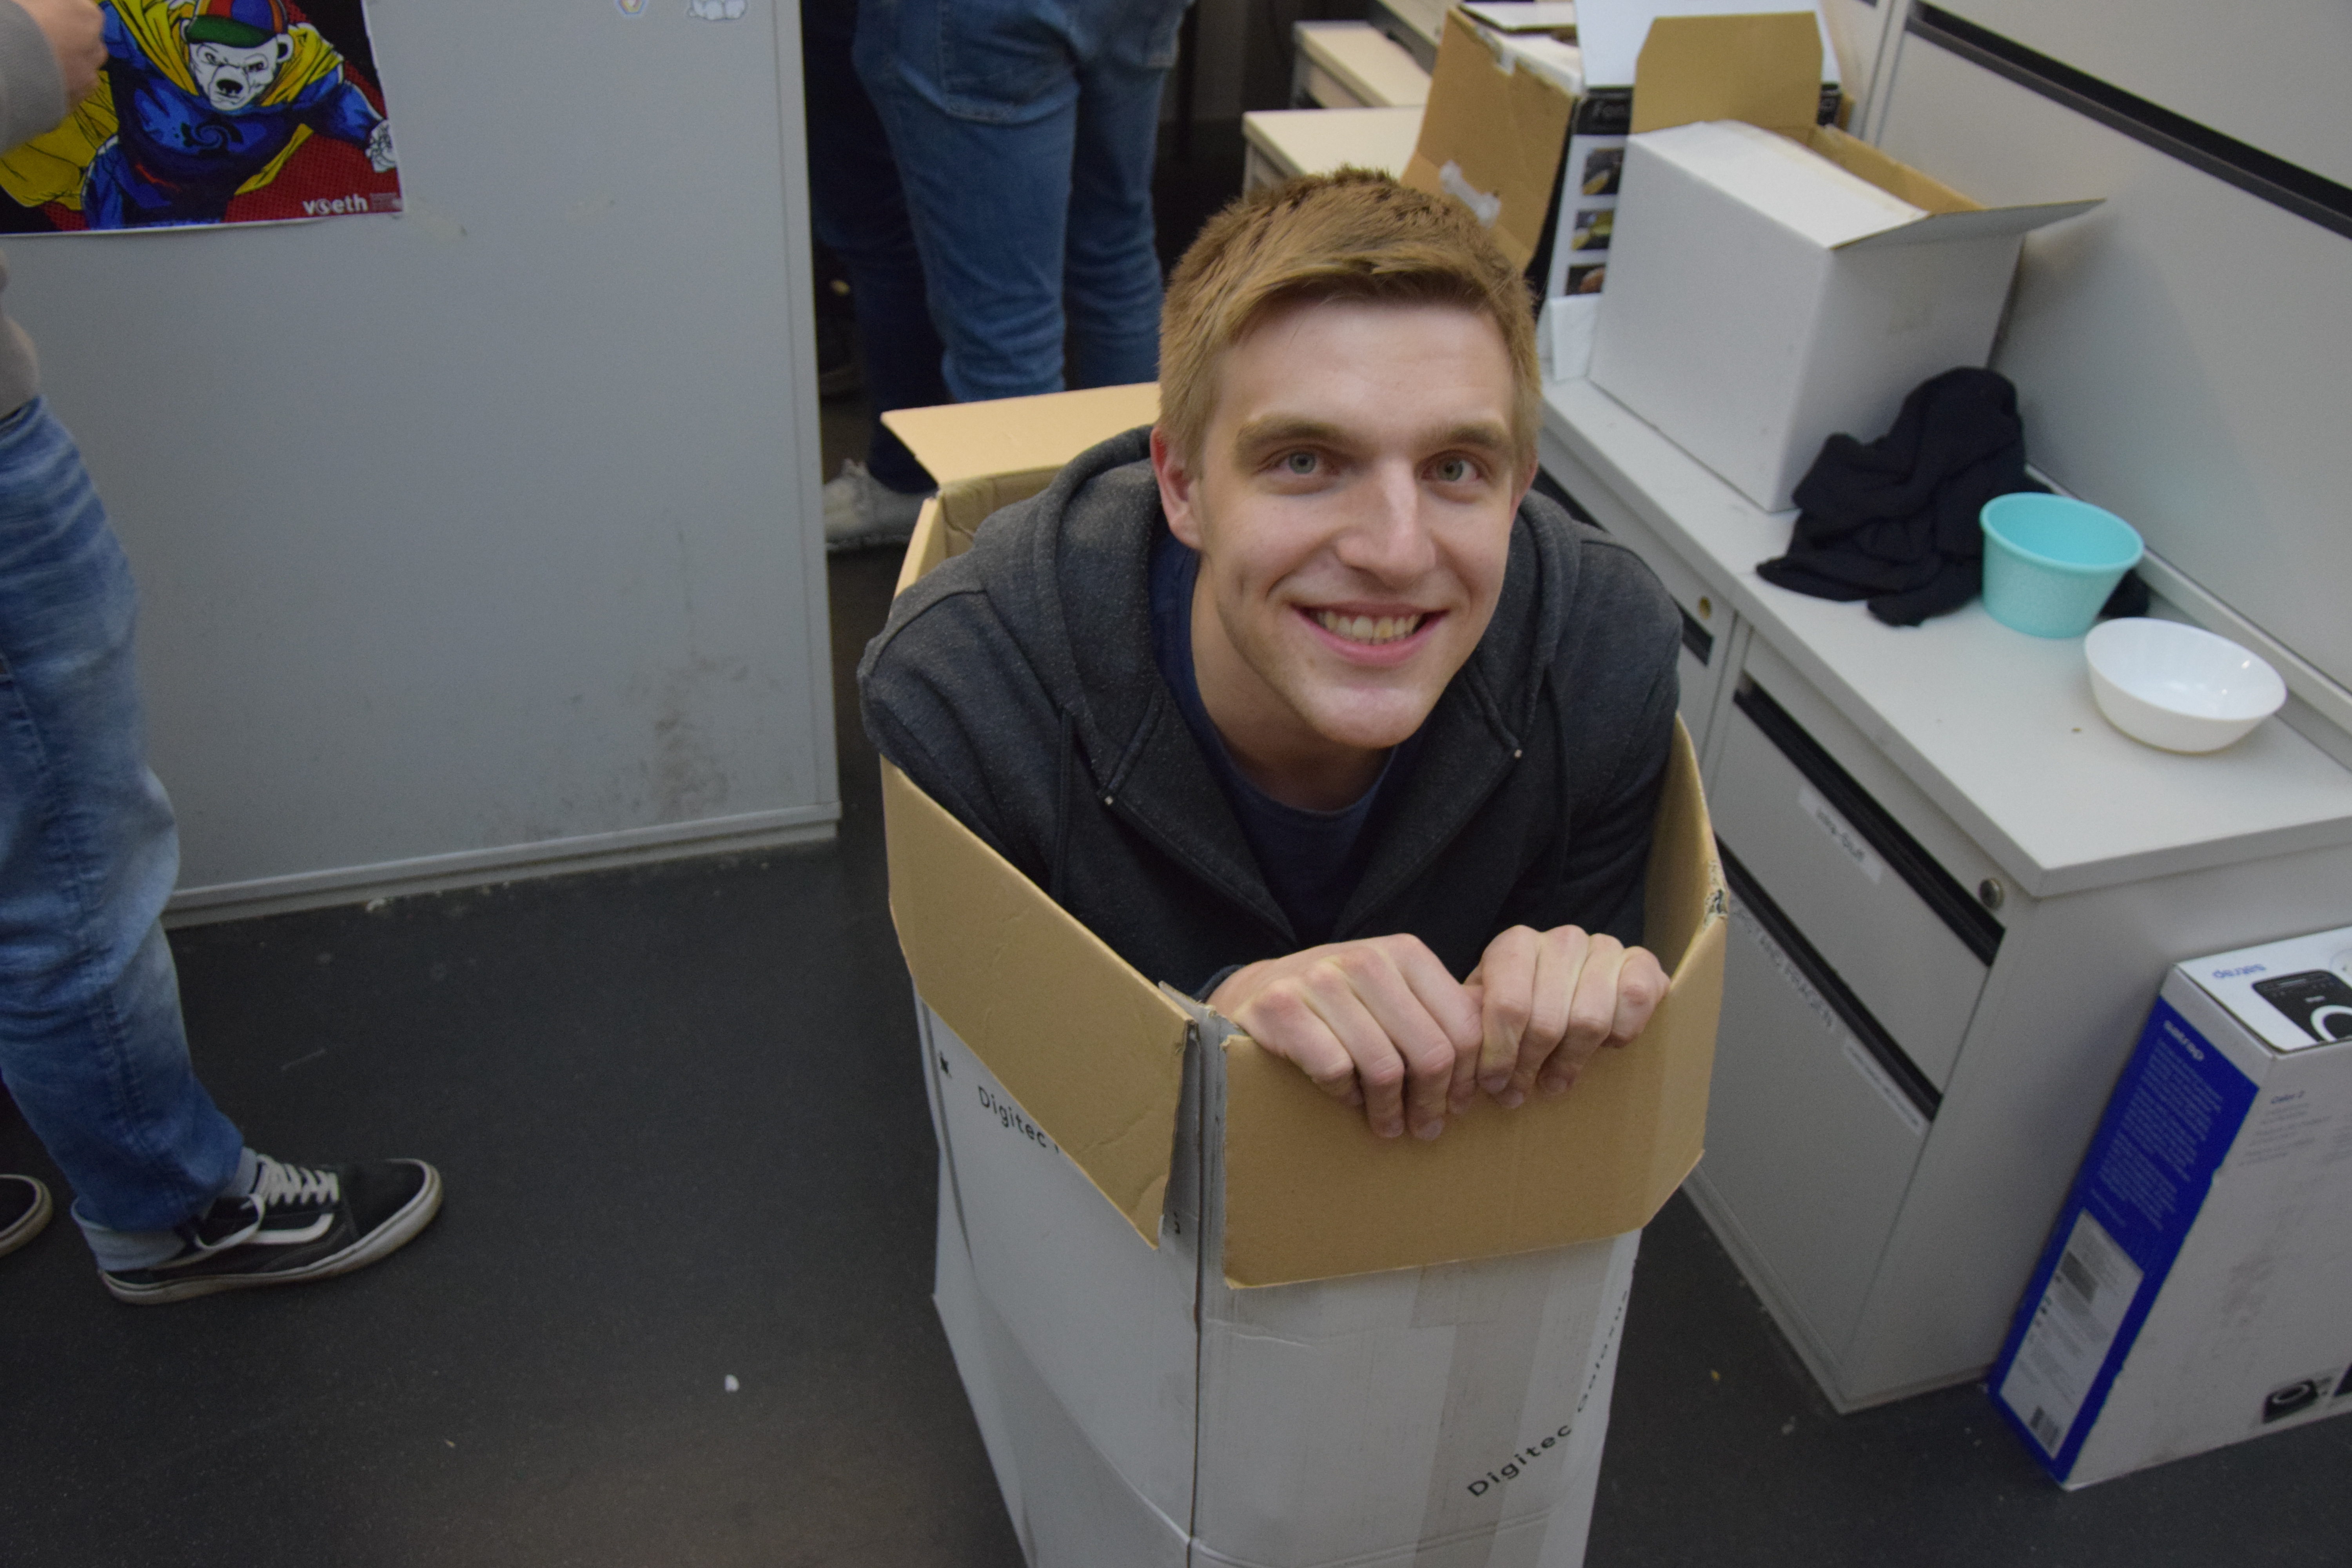
\includegraphics[width=\linewidth]{../images/DSC_0147.JPG}}

  
\section{Section with a number}
Phasellus fringilla. Aliquam mollis tellus vel odio. Vestibulum ante ipsum primis in faucibus orci luctus et ultrices posuere cubilia
Curae; Vestibulum gravida sapien sed diam dictum pharetra. Nulla ac odio. Duis vitae metus ut purus feugiat interdum. Duis eros enim, tincidunt ac, venenatis et, dignissim id, lacus. Curabitur sagittis dolor nec augue. Sed ultricies mauris. Donec semper, enim eu vestibulum placerat, justo risus eleifend quam, ac semper velit pede convallis arcu.

\subsection{Other details relating to the presentation of your aricle}
\begin{itemize}[leftmargin=12bp,itemsep=0bp,topsep=0bp]
  \item The page number is not added, but expect it to be in the lower corners of a spread.
  \item This template assumese that your article starts on the left page of a spread. If you want it to start on the right page, uncomment the two lines right under the beginning of the document. Make sure that the editorial team is aware of your preferences for article start so that there are no misunderstandings.
  \item You are not obliged to use all elements of this template. Play around with them, and feel free to exclude elements if you don't find them fitting with the message of your content.
  \item Try to make sure that your article's final page has the top 50\% filled with content. Otherwise, there's an awkward break and, unlike blitz, we can't really immediately proceed with the next article.
\end{itemize}

\section*{Good luck and have fun writing!}

\end{document}
